\ifdefined\pdfoutput\pdfoutput=1\fi % forces arXiv to process this file with pdflatex instead of DVI-producing "latex"; see README section "Final submission"
% This template has been tested with LLNCS DOCUMENT CLASS -- version 2.21 (12-Jan-2022)

% !TeX spellcheck = en-US
% LTeX: language=en-US
% !TeX encoding = utf8
% !TeX program = lualatex
% !BIB program = bibtex
% -*- coding:utf-8 mod:LaTeX -*-
%
% vvvvvvvv  The content starts in line 704 (\begin{document}); the first
%           heading (\section{Introduction}) is in line 743.
%           Everything above is the preamble: document class, packages, and settings.

% "a4paper" enables:
%
%  - easy print out on DIN A4 paper size
%
% One can configure default page size (a4 vs. letter) in the LaTeX installation.
% Thus, it is configuration dependent, what the paper size will be.
% Having "a4paper" option present, the page size is set to A4.
% Note that the current word template offered by Springer is DIN A4.
%
% "runningheads" enables:
%
%  - page number on page 2 onwards
%  - title/authors on even/odd pages
%
% This is good for other readers to enable proper archiving among other papers and pointing to
% content. Even if the title page states the title, when printed and stored in a folder, when
% blindly opening the folder, one could hit not the title page, but an arbitrary page. Therefore,
% it is good to have title printed on the pages, too.
%
% The option "runningheads" needs to be removed upon request of the publisher.
%
% To disable outputting page headers and footers, remove "runningheads"
\documentclass[runningheads,a4paper,english]{llncs}[2022/01/12]

\usepackage{iftex}

% backticks (`) are rendered as such in verbatim environments.
% See the following links for details:
%   - https://tex.stackexchange.com/a/341057/9075
%   - https://tex.stackexchange.com/a/47451/9075
%   - https://tex.stackexchange.com/a/166791/9075
\usepackage{upquote}

% Set English as the language and allow to write hyphenated"=words
%
% Even though `american`, `english` and `USenglish` are synonyms for babel package (according to https://tex.stackexchange.com/questions/12775/babel-english-american-usenglish), the llncs document class is prepared to avoid the overriding of certain names (such as "Abstract." -> "Abstract" or "Fig." -> "Figure") when using `english`, but not when using the other 2.
% english has to go last to set it as the default language
\usepackage[ngerman,main=english]{babel}
%
% Hint by http://tex.stackexchange.com/a/321066/9075 -> enable "= as dashes
\addto\extrasenglish{\languageshorthands{ngerman}\useshorthands{"}}

% Links behave as they should. Enables "\url{...}" for URL typesettings.
% Allow URL breaks also at a hyphen, even though it might be confusing: Is the "-" part of the address or just a hyphen?
% See https://tex.stackexchange.com/a/3034/9075.
\usepackage[hyphens]{url}

% When activated, use text font as URL font, not the monospaced one.
% For all options see https://tex.stackexchange.com/a/261435/9075.
% \urlstyle{same}

% Allow URL breaks after any character, so that long URLs do not run into the margin.
% Loaded before biblatex, so that the biblatex settings of the URL penalties stay.
% See https://ctan.org/pkg/xurl.
\usepackage{xurl}

% nicer // - solution by http://tex.stackexchange.com/a/98470/9075
% DO NOT ACTIVATE -> prevents line breaks
%\makeatletter
%\def\Url@twoslashes{\mathchar`\/\@ifnextchar/{\kern-.2em}{}}
%\g@addto@macro\UrlSpecials{\do\/{\Url@twoslashes}}
%\makeatother

%% !!! If you change the font, be sure that words such as "workflow" can
%% !!! still be copied from the PDF. If this is not the case, you have
%% !!! to use glyphtounicode (pdflatex only). See the comment at \input{glyphtounicode}.
%%
%% Background: "workflow" contains "fl" which is a ligature, which in turn
%%             is rendered as one character in the PDF and needs to be split
%%             whily copying.

\ifluatex
  \usepackage[no-math]{fontspec}
  \usepackage{unicode-math}

  % Typewriter font (for source code etc)
  % Use New Computer Modern font (Computer Modern is the default LaTeX font; this is the implemented modern variant)
  % Source: https://tug.org/FontCatalogue/newcomputermoderntypewriter/

  \setmainfont[
    ItalicFont=NewCM10-Italic.otf,
    BoldFont=NewCM10-Bold.otf,
    BoldItalicFont=NewCM10-BoldItalic.otf,
    SmallCapsFeatures={Numbers=OldStyle}]{NewCM10-Regular.otf}

  \setsansfont[
    ItalicFont=NewCMSans10-Oblique.otf,
    BoldFont=NewCMSans10-Bold.otf,
    BoldItalicFont=NewCMSans10-BoldOblique.otf,
    SmallCapsFeatures={Numbers=OldStyle}]{NewCMSans10-Regular.otf}

  \setmonofont[ItalicFont=NewCMMono10-Italic.otf,
    BoldFont=NewCMMono10-Bold.otf,
    BoldItalicFont=NewCMMono10-BoldOblique.otf,
    SmallCapsFeatures={Numbers=OldStyle}]{NewCMMono10-Regular.otf}

  \setmathfont{NewCMMath-Regular.otf}

  % Enable proper ligatures for English documents (German documents use autotype, see ADR-0008)
  % For more information see https://ctan.org/pkg/selnolig
  \usepackage{selnolig}

\else
  % This is the modern package for "Computer Modern".
  % In case this gets activated, check that ligatures can still be copied (pdflatex: glyphtounicode)
  \usepackage[%
    rm={oldstyle=false,proportional=true},%
    sf={oldstyle=false,proportional=true},%
    % By using 'variable=true' the monospaced font can be used as variable font (with different widths per letter)
    % However, this makes listings look ugly.
    tt={oldstyle=false,proportional=true,variable=false},%
    qt=false%
  ]{cfr-lm}

  % Has to be loaded AFTER any font packages. See https://tex.stackexchange.com/a/2869/9075.
  \usepackage[T1]{fontenc}
\fi

% Character protrusion and font expansion. See http://www.ctan.org/tex-archive/macros/latex/contrib/microtype/

\usepackage[
  babel=true, % Enable language-specific kerning. Take language-settings from the language of the current document (see Section 6 of microtype.pdf)
  expansion=alltext,
  protrusion=alltext-nott, % Ensure that at listings, there is no change at the margin of the listing
  % In the standard configuration, this template is always in the final mode, so this option only makes a difference if "pros" use the draft mode
  final % Always enable microtype, even if in draft mode. This helps finding bad boxes quickly.
]{microtype}

% \texttt{test -- test} keeps the "--" as "--" (and does not convert it to an en dash)
\DisableLigatures{encoding = T1, family = tt* }

%\DeclareMicrotypeSet*[tracking]{my}{ font = */*/*/sc/* }%
%\SetTracking{ encoding = *, shape = sc }{ 45 }
% Source: http://homepage.ruhr-uni-bochum.de/Georg.Verweyen/pakete.html
% Deactiviated, because does not look good

% Avoid orphans and widows (a single line of a paragraph left at the bottom or top
% of a page).
\ifdefined\directlua
  % LuaLaTeX: lua-widow-control removes them by lengthening or shortening a paragraph
  % by one line, instead of leaving an empty line at the bottom of the page.
  \usepackage{lua-widow-control}
\else
  % pdfLaTeX: nowidow sets \clubpenalty and \widowpenalty; using a package feels less
  % hacky than tuning them manually.
  \usepackage[all,defaultlines=3]{nowidow}
\fi

% Avoid a widow line being split off a displayed equation.
\displaywidowpenalty=10000

% Avoid a lone short word (or hyphenated fragment) as the last line of a paragraph.
% LuaTeX only: impnattypo's lastparline feature vetoes the offending line break in
% each affected paragraph. The package's pdfTeX fallback instead stretches
% \parfillskip globally, which loosens interword spacing everywhere -- the reason
% the package was once reverted, see
% https://github.com/latextemplates/lncs-enhanced/issues/16
\ifdefined\directlua
  \usepackage[lastparline]{impnattypo}
\fi

% --- Rectangular ("block") paragraphs -------------------------------------
% When enabled, the last line of every paragraph is stretched to the full
% column width, so each paragraph forms a perfect rectangle. This is
% demanding typography: paragraphs whose last line is naturally short get
% visibly wide interword spaces, and good results usually require rewording
% sentences until every paragraph fits (copy fitting). The lone-word tweak
% above (impnattypo) becomes irrelevant while this is active.
% Enable by uncommenting the \rectangularparagraphstrue line:
\newif\ifrectangularparagraphs
%\rectangularparagraphstrue
\ifrectangularparagraphs
  \setlength{\parfillskip}{0pt}      % force the last line to reach the margin
  \setlength{\emergencystretch}{3em} % soften overfull lines this may cause
\fi

\usepackage{graphicx}

% Smaller PDF: graphicscache re-encodes every included image once with Ghostscript (lossless, at most 300 dpi) and
% caches the result in graphicscache/. It needs shell escape and an external pdflatex, so it is loaded only when the
% document is compiled with --shell-escape; without, images are embedded as they are.
% Doc: https://ctan.org/pkg/graphicscache
\ExplSyntaxOn
\sys_if_shell_unrestricted:T { \RequirePackage [ compress = flat ] { graphicscache } }
\ExplSyntaxOff
\makeatletter
% graphicscache spells the Ghostscript filter "FlatEncode"; Ghostscript knows it as FlateEncode and rejects the typo.
% Remove when https://github.com/xqms/graphicscache/issues/30 is fixed.
\@ifpackageloaded{graphicscache}{%
  \def\graphicscache@compress@mode{FlateEncode}%
  % graphicscache parses the \includegraphics options itself and does not know graphicx's alt text (the markdown package sets it).
  % Remove when https://github.com/xqms/graphicscache/issues/29 is fixed.
  \pgfkeys{/graphicscache/alt/.code={\graphicscache@addarg{alt={\unexpanded{#1}}}}}%
}{}
\makeatother

% Diagonal lines in a table - http://tex.stackexchange.com/questions/17745/diagonal-lines-in-table-cell
% Slashbox is not available in texlive (due to licensing) and also gives bad results. Thus, we use diagbox
\usepackage{diagbox}

\usepackage[dvipsnames, table]{xcolor}
% See https://github.com/gpoore/minted
\usepackage[newfloat]{minted}

\setminted{
  % Line numbers not flowing out of the margin
  numbersep=5pt,
  xleftmargin=12pt,
  %
  % Better listing breaking
  breakafter=-/\{,
  breakbefore=\\
  %
  % Alternative: Rely on pygment's tokenizer. Does not work well with LaTeX and comments
  % breakbytoken=true,
  % breakbytokenanywhere=true
}

%\usemintedstyle{bw} %black and white style
%\usemintedstyle{vs} %visual studio
\usemintedstyle{friendly_grayscale}
%\usemintedstyle{friendly}
%\usemintedstyle{eclipse} %http://www.jevon.org/wiki/Eclipse_Pygments_Style
%\usemintedstyle{autumn}
%\usemintedstyle{rrt}
%\usemintedstyle{borland}

% A paper keeps the caption style of its document class: the caption package would change it (e.g., "Figure 1:" instead of IEEE's "Fig. 1.")
\SetupFloatingEnvironment{listing}{name=List.,within=none}

% When using both minted and listings
% Compatibility of packages minted and listings with respect to the numbering of "List." caption
% Source: https://tex.stackexchange.com/a/269510/9075
% \AtBeginEnvironment{listing}{\setcounter{listing}{\value{lstlisting}}}
% \AtEndEnvironment{listing}{\stepcounter{lstlisting}}

% Enable \label in listing lines (via escapeinside) and referencing them using \zcref, e.g., "Line 2".
% fancyvrb steps the line counter without \refstepcounter: no counter for \zcref and no target for the hyperlink.
% See https://github.com/gusbrs/zref-clever/issues/65 and https://tex.stackexchange.com/q/132420/9075.
\makeatletter
\def\FV@refstepcounter#1{%
  \refstepcounter{#1}%
  \protected@edef\@currentlabel{\csname p@#1\endcsname\arabic{#1}}%
}
% Unique hyperlink targets in each listing
\newcounter{FancyVerbListing}
\let\FV@StepLineNo@orig\FV@StepLineNo
\def\FV@StepLineNo{\stepcounter{FancyVerbListing}\FV@StepLineNo@orig}
\def\theHFancyVerbLine{\arabic{FancyVerbListing}.\arabic{FancyVerbLine}}
\makeatother

% For easy quotations: \enquote{text}
% This package is very smart when nesting is applied, otherwise textcmds (see below) provides a shorter command
\usepackage[autostyle=true]{csquotes}

% Enable using "`quote"' - see https://tex.stackexchange.com/a/150954/9075
\defineshorthand{"`}{\openautoquote}
\defineshorthand{"'}{\closeautoquote}

% Nicer tables (\toprule, \midrule, \bottomrule)
\usepackage{booktabs}

% Extended enumerate, such as \begin{compactenum}
\usepackage{paralist}

% Bibliopgraphy enhancements
%  - enable \cite[prenote][]{ref}
%  - enable \cite{ref1,ref2}
% Alternative: \usepackage{cite}, which enables \cite{ref1, ref2} only (otherwise: Error message: "White space in argument")

% Doc: http://texdoc.net/natbib
\usepackage[%
  square,        % for square brackets
  comma,         % use commas as separators
  numbers,       % for numerical citations;
  %sort           % orders multiple citations into the sequence in which they appear in the list of references;
  sort&compress  % as sort but in addition multiple numerical citations are compressed if possible (as 3-6, 15);
]{natbib}

% In the bibliography, references have to be formatted as 1., 2., ... not [1], [2], ...
\renewcommand{\bibnumfmt}[1]{#1.}

% "A and B" (two authors, \citet) follows the document language: splncs04nat.bst writes \andname{} instead of "and".
% babel has no caption for "and", so register one; \andname then switches with the language like \figurename.
\setlocalecaption{english}{and}{and}
\setlocalecaption{ngerman}{and}{und}

% Enable hyperlinked author names in the case of \citet
% Source: https://tex.stackexchange.com/a/76075/9075
\usepackage{etoolbox}
\makeatletter
\patchcmd{\NAT@test}{\else \NAT@nm}{\else \NAT@hyper@{\NAT@nm}}{}{}
\makeatother

% To embed the bibliography into the PDF (readers can extract it, e.g., with JabRef via "Import into library" on the PDF), uncomment:
%\usepackage{embedfile}
%\embedfile[mimetype=application/x-bibtex,desc=BibTeX entries of all references]{paper.bib}

% Self-archiving version (e.g., for your homepage): uncomment the following lines and fill in the data of the publication.
% The package adds the copyright notice of the publisher and a link to the published version, see https://ctan.org/pkg/authorarchive.
%\usepackage[LNCS]{authorarchive}
%\authorsetup{
%  key={lastname-paper-YYYY},                 % basename of the PDF (and of the .bib file)
%  year={YYYY},
%  publication={Proceedings of the Conference},
%  startpage={1},
%  doi={10.0000/00000},
%  baseurl={https://www.example.org/papers}, % where you publish the PDF
%  nobib,                                    % remove to embed <key>.bib (the BibTeX entry of this paper) into the PDF
%  nocopyright,                              % usual case for LNCS
%}

% Prepare more space-saving rendering of the bibliography
% Source: https://tex.stackexchange.com/a/280936/9075
\SetExpansion
[ context = sloppy,
  stretch = 30,
  shrink = 60,
  step = 5 ]
{ encoding = {OT1,T1,TS1} }
{ }

% Put figures aside a text
% Even though the package is from 1998, it works well
\usepackage[rflt]{floatflt}

% Colored tables
% --------------
% xcolor loads the package colortbl
%
% Extended functions within tables
% --------------------------------
%%% Doc: http://mirror.ctan.org/tex-archive/macros/latex/contrib/multirow/multirow.sty
\usepackage{multirow} % cells spanning multiple rows
%
%%% Doc: Documentation inside dtx Package
\usepackage{dcolumn}  % alignment at the decimal separator
%
%%% Doc: https://texdoc.org/serve/tablefootnote/0
\usepackage{tablefootnote} % \tablefootnote: a footnote inside a floating table (plain \footnote is lost there)

% A bit more space between the rows of a table (\extrarowheight is provided by array, which dcolumn loads)
\setlength{\extrarowheight}{1pt}

%%% Doc: http://mirror.ctan.org/tex-archive/macros/latex/contrib/supertabular/supertabular.pdf
%\usepackage{supertabular}

% tikz / pgfplots stack used by the "Figures with tikz" and "Plots with pgfplots"
% examples. Loading pgfplots pulls in tikz.
\usepackage{pgfplots}
\pgfplotsset{compat=1.18}

% longtable: tables that automatically break across page boundaries.
\usepackage{longtable}

%%% Footnotes/Endnotes ===================================================

% Save space: set all footnotes of a page side by side in one paragraph (LuaLaTeX only).
% pdfLaTeX cannot break URLs inside such footnotes: footmisc collects each footnote in a box, and TeX adds no break points
% to math (which \url uses) inside a box. LuaTeX's \mathpenaltiesmode does.
%\usepackage[para]{footmisc}
%\mathpenaltiesmode=1

% Put footnotes below floats
% Source: https://tex.stackexchange.com/a/32993/9075
\usepackage{stfloats}
\fnbelowfloat

% Extended support for footnotes
%
%\usepackage{dblfnote}  % Two-column footnotes
%
% No superscript numbers in the footnote (KOMA-Script-specific):
%\deffootnote[1.5em]{0pt}{1em}{\makebox[1.5em][l]{\bfseries\thefootnotemark}}
%
% Increase the spacing between footnotes:
%\setlength{\footnotesep}{.85\baselineskip}
%
% Following command disables the separating line of the footnote
%\renewcommand{\footnoterule}{}
%
%\addtolength{\skip\footins}{\baselineskip} % Spacing text <-> footnote

% Always place footnotes at the very bottom on a \raggedbottom page
% fnpos comes from the yafoot package
%\usepackage{fnpos}
%\makeFNbelow
%\makeFNbottom

% TODO (and comment) configuration
%
% - \todo (from todo, easy-todo, todonotes) / \TODO (from fixmetodonotes) - for "normal" TODOs
% - \todofix - "important" TODOs
%
% - \textcomment - highlights text and has a hover comment
% - \sidecomment - just puts a comment to the side. Note: \comment MUST NOT be used as command name, it is already defined by much packages (mathdesign, mindflow, verbatim, and others)
%
% - \missingfigure
%
% - \textmarker
% - \modified
% - \change      - addresses a review comment

% Enable nice comments
\usepackage{pdfcomment}

\ifdefined\directlua
  % Highlighting that breaks across lines (\colorbox does not): lua-ul's \highLight; the color needs luacolor
  \usepackage{luacolor,lua-ul}
  \newcommand{\textcomment}[2]{\highLight[yellow!60]{#1}\pdfcomment[color={0.234 0.867 0.211},hoffset=-6pt,voffset=10pt,opacity=0.5]{#2}}
\else
  \newcommand{\textcomment}[2]{\colorbox{yellow!60}{#1}\pdfcomment[color={0.234 0.867 0.211},hoffset=-6pt,voffset=10pt,opacity=0.5]{#2}}
\fi

% Small PDF comment
% 1st parameter: comment
\newcommand{\sidecomment}[1]{\pdfcomment[color={0.045 0.278 0.643},voffset=4pt,icon=Note]{#1}}
% Disabled variant - for the final PDF
%\newcommand{\sidecomment}[1]{}

\newcommand{\todo}[1]{TODO!\sidecomment{#1}}

% Changes
%
% 1st parameter: review comment
% 2nd parameter: new text
\newcommand{\change}[2]{{\color{red}#2}\pdfcomment[color={0.234 0.867 0.211},voffset=8pt,opacity=0.5]{#1}}
% Disabled variant - for the final PDF
%\newcommand{\change}[2]{#2}

% Define default commands
\makeatletter
\@ifundefined{missingfigure}{\newcommand{\missingfigure}{... missing figure ...}}{}
\@ifundefined{textcomment}{\newcommand{\textcomment}[2]{#1 \todo{#2}}}{}
\@ifundefined{sidecomment}{\newcommand{\sidecomment}[1]{\marginpar{#1}}}{}
\@ifundefined{todo}{\newcommand{\todo}[1]{\sidecomment{#1}}}{}
\@ifundefined{TODO}{\newcommand{\TODO}[1]{\todo{#1}}}{}
\@ifundefined{todofix}{\newcommand{\todofix}[1]{\todo{#1}}}{}
\@ifundefined{change}{\newcommand{\change}[2]{#1 $\rightarrow$ #2}}{}
\makeatother

% Textmarker (Textfarbe rot)
\newcommand{\textmarker}[1]{{\color{red} #1}\xspace}

% Modified (Text blau)
\newcommand{\modified}[1]{{\color{blue!60!black} #1}\xspace}

% Edits and comments by several authors, each with their own color and initials (phfcc)
% Doc: https://ctan.org/pkg/phfcc
\usepackage{phfcc}
\ifdefined\directlua
  \phfSetDefaultCommentingStyle{style=rmstrikethrough} % strike through removed text across lines (LuaLaTeX only)
\fi
% Comments as footnotes keep the layout intact, e.g., to check page limits
%\phfSetDefaultCommentingStyle{style=footcomments}
% One command per author: \FA{added text}, \FA*{text to remove}, \FA[a comment], \FA!{important};
% the initials appear once per page in the margin; the forms do not combine (\FA*[...]{...} is only a comment), so
% write \FA*{removed}\FA[comment]. Add one line per further author with their initials.
\phfMakeCommentingCommand[initials={FA}]{FA} % first author
% Final version: hide all edits and comments (there is no class option for it: "final" is the default of every class)
%\phfDisableCommentingCommands

\usepackage[group-minimum-digits=4,per-mode=fraction]{siunitx}

% Write text in Markdown instead of LaTeX: \begin{markdown} ... \end{markdown}, or \markdownInput{chapter.md} for a whole file.
% Doc: https://ctan.org/pkg/markdown
% LuaLaTeX only: under pdfLaTeX, the package needs --shell-escape.
\ifluatex
  \usepackage[
    citations,          % [@key] citation syntax
    hybrid,             % pass raw LaTeX through
    notes,              % [^label] referenced footnotes
    inlineNotes,        % ^[inline footnote text]
    pipeTables,         % | a | b | style tables
    tableCaptions,      % : Caption text below a table
    tableAttributes,    % {#id} identifier on a table caption
    headerAttributes,   % {#id} identifier on a heading
    relativeReferences, % <#id> to reference an id defined via {#id} (typeset by \zcref, see below)
    hashEnumerators,    % 1) 2) 3) style enumerators
  ]{markdown}
  % The markdown package typesets "#" as \chapter if the class defines it (llncs does); in a paper, "#" is a section
  % textidote: ignore begin
  \renewcommand{\markdownRendererHeadingOne}[1]{\section{#1}}
  \renewcommand{\markdownRendererHeadingTwo}[1]{\subsection{#1}}
  \renewcommand{\markdownRendererHeadingThree}[1]{\subsubsection{#1}}
  % textidote: ignore end
  % Markdown's own reference syntax <#id> typesets the bare number (\ref).
  % Typeset it with \zcref instead, so that "<#tbl:example> shows" reads "Table 1 shows".
  % Other links are rendered as before.
  \ExplSyntaxOn
  \cs_new_protected:Npn \ltg_markdown_link:nnnn #1#2#3#4
  {
    \tl_set:Nx \l_tmpa_tl { \tl_range:nnn {#3} { 1 } { 1 } }
    \bool_lazy_all:nTF
    {
      { \str_if_eq_p:nn {#1} {#2} }
      { \str_if_eq_p:VV \l_tmpa_tl \c_hash_str }
      { \tl_if_empty_p:n {#4} }
    }
    { \exp_args:Nx \zcref { \tl_range:nnn {#3} { 2 } { -1 } } }
    { \markdownRendererLinkPrototype {#1} {#2} {#3} {#4} }
  }
  \markdownSetup{ renderers = { link = { \ltg_markdown_link:nnnn {#1} {#2} {#3} {#4} } } }
  \ExplSyntaxOff
\fi

% Enable that parameters of \zcref{}, \ref{}, \cite{}, ... are linked so that a reader can click on the number an jump to the target in the document
\usepackage{hyperref}

% Enable hyperref without colors and without bookmarks
\hypersetup{
  hidelinks,
  colorlinks=true,       % Links erhalten Farben statt Kaeten
  raiselinks=true,       % calculate real height of the link
  allcolors=black,
  pdfstartview=Fit,
  breaklinks=true,       % Links ueberstehen Zeilenumbruch
  hypertexnames=false,   % Fix jumping to algorithm line - http://tex.stackexchange.com/a/156404/9075
}

% Enable correct jumping to figures when referencing
\usepackage[all]{hypcap}

% Show how far each chapter or section is written:
% \progress{60} below a heading draws a bar filled to 60 %.
% Set \showprogressfalse to hide all bars, e.g., for the submitted version.
% To use it, uncomment the following lines.
% \usepackage{progressbar}
% \newif\ifshowprogress
% \showprogresstrue
% \newcommand{\progress}[1]{%
%   \ifshowprogress
%     \par\vspace{-.5\baselineskip}%
%     {\parfillskip=0pt\noindent\progressbar[width=\linewidth,heighta=4pt,borderwidth=0.4pt,subdivisions=4,filledcolor=black!50]{\fpeval{#1/100}}\par}%
%   \fi
% }

\usepackage[caption=false,font=footnotesize]{subfig}

% Alternative for making subfigures:
% Part of the caption package. See http://www.ctan.org/pkg/caption
% Replaces the subfigure and subfig packages - see https://tex.stackexchange.com/a/13778/9075
%
% (subfigure is outdated. subfig is maintained, but subcaption is better)
% See: http://tex.stackexchange.com/questions/13625/subcaption-vs-subfig-best-package-for-referencing-a-subfigure
%\usepackage[hypcap=true]{subcaption}

\usepackage{mindflow}

% Extensions for references inside the document (\zcref{fig:sample}, ...)
% Use \zcref{...} (and \Zcref{...} at the beginning of a sentence) instead of \ref: Type of reference included in the link
% That means, "Figure 5" is a full link instead of just "5".
% The names follow the document language (babel); zref-clever is compatible with tagged PDFs.
% Each \label also sets a zref label, so \zcref works with standard \label.
\usepackage{zref-clever}
\zcsetup{cap, nameinlink=true, abbrev}
% \Zcref{...} is short for \zcref[S]{...}: capitalized, unabbreviated name at the beginning of a sentence
\NewDocumentCommand{\Zcref}{s O{} m}{\IfBooleanTF{#1}{\zcref*[S,#2]{#3}}{\zcref[S,#2]{#3}}}
% Lines of minted listings are referenced as "Line 2"
\zcsetup{countertype={FancyVerbLine=line}}
\zcLanguageSetup{english}{
  type=section, Name-sg-ab=Sect., Name-pl-ab=Sect.,
  type=listing, Name-sg-ab=List., Name-pl-ab=List.,
}

\usepackage{lipsum}

% For demonstration purposes only
% These packages can be removed when all examples have been deleted
\usepackage[math]{blindtext}
\usepackage{mwe}
\usepackage{hologo} % logos such as \hologo{LuaLaTeX} (used in the Markdown example)
\usepackage[realmainfile]{currfile}
\usepackage{tcolorbox}
\tcbuselibrary{minted}
% Required for proper example rendering in the compiled PDF
\newcount\LTGbeginlineexample
\newcount\LTGendlineexample
\newenvironment{ltgexample}%
{\LTGbeginlineexample=\numexpr\inputlineno+1\relax}%
{\LTGendlineexample=\numexpr\inputlineno-1\relax%
  \tcbinputlisting{%
    listing only,
    listing file=\currfilepath,
    colback=green!5!white,
    colframe=green!25,
    coltitle=black!90,
    coltext=black!90,
    left=8mm,
    title=Corresponding \LaTeX{} code of \texttt{\currfilepath},
    minted language=TeX,
    minted style=vs,
    minted options={
        fontsize=\footnotesize,
        firstline=\the\LTGbeginlineexample,
        lastline=\the\LTGendlineexample,
        firstnumber=\the\LTGbeginlineexample,
        breaklines,
        linenos,
        numbersep=8pt
      }
  }
}%

%introduce \powerset - hint by http://matheplanet.com/matheplanet/nuke/html/viewtopic.php?topic=136492&post_id=997377
\DeclareFontFamily{U}{MnSymbolC}{}
\DeclareSymbolFont{MnSyC}{U}{MnSymbolC}{m}{n}
\DeclareFontShape{U}{MnSymbolC}{m}{n}{
  <-6>    MnSymbolC5
  <6-7>   MnSymbolC6
  <7-8>   MnSymbolC7
  <8-9>   MnSymbolC8
  <9-10>  MnSymbolC9
  <10-12> MnSymbolC10
  <12->   MnSymbolC12%
}{}
\DeclareMathSymbol{\powerset}{\mathord}{MnSyC}{180}

% Allows for defining commands that don't eat spaces.
\usepackage{xspace}
% Adds compatibility to \xspace und \enquote
\makeatletter
\xspaceaddexceptions{\grqq \grq \csq@qclose@i \} }
\makeatother

\newcommand{\eg}{e.g.,\ }
\newcommand{\ie}{i.e.,\ }

% Enable hyphenation at other places as the dash.
% Example: application\hydash specific
\makeatletter
\newcommand{\hydash}{\penalty\@M-\hskip\z@skip}
% Definition of "= taken from http://mirror.ctan.org/macros/latex/contrib/babel-contrib/german/ngermanb.dtx
\makeatother

% Add manual adapted hyphenation of English words
% See https://ctan.org/pkg/hyphenex and https://tex.stackexchange.com/a/22892/9075 for details
\input{ushyphex}

% correct bad hyphenation here
\hyphenation{
  op-tical net-works semi-conduc-tor
  % May not be hypphenated
  AROMA TOSCA BPMN OASIS OMG DMTF IT DevOps
}

% lccaps provides \textlcc (lowercase caps), used by \initialism in commands.tex.
% Doc: https://ctan.org/pkg/lccaps
\usepackage{lccaps}
\input{commands}

% Add copyright
%
% This is recommended if you intend to send the version to colleagues
% See https://ctan.org/pkg/llncsconf for details
\iffalse
  % state: intended | submitted | llncs
  % you can add "crop" if the paper should be cropped to the format Springer is publishing
  \usepackage[intended]{llncsconf}

  \conference{name of the conference}

  % in case of "proceedings" (final version!)
  % example: \llncs{Anonymous et al. (eds). \emph{Proceedings of the International Conference on \LaTeX-Hacks}, LNCS~42. Some Publisher, 2016.}{0042}
  % 0042 denotes an example start page
  \llncs{book editors and title}{0042}
\fi

\ifpdftex
  % Enable copy and paste of text from the PDF
  % Only required for pdflatex. It "just works" in the case of lualatex.
  % Alternative: cmap or mmap package
  % mmap enables mathematical symbols but does not work with the newtx font set
  % See: https://tex.stackexchange.com/a/64457/9075
  % Other solutions outlined at http://goemonx.blogspot.de/2012/01/pdflatex-ligaturen-und-copynpaste.html and http://tex.stackexchange.com/questions/4397/make-ligatures-in-linux-libertine-copyable-and-searchable
  % Troubleshooting outlined at https://tex.stackexchange.com/a/100618/9075
  %
  % According to https://tex.stackexchange.com/q/451235/9075 this is the way to go
  \input{glyphtounicode}
  \pdfgentounicode=1
\fi
% LuaLaTeX: avoid lines running into the margin. linebreaker sets an overfull
% paragraph again with increasing \tolerance and \emergencystretch until it fits.
% Loaded at the end of the preamble, after all packages that change line breaking.
% See https://ctan.org/pkg/linebreaker.
\ifdefined\directlua
  \usepackage{linebreaker}
\fi

\begin{document}

\title{Paper Title}
% If Title is too long, use \titlerunning
%\titlerunning{Short Title}

% Single institute
\author{Firstname Lastname \and Firstname Lastname}

% If there are too many authors, use \authorrunning
%\authorrunning{First Author et al.}

\institute{Institute}

%% Multiple institutes - ALTERNATIVE to the above
% \author{%
%     Firstname Lastname\inst{1} \and
%     Firstname Lastname\inst{2}
% }
%
%If there are too many authors, use \authorrunning
%  \authorrunning{First Author et al.}
%
%  \institute{
%      Institute 1\\
%      \email{...}\and
%      Institute 2\\
%      \email{...}
%}

\maketitle

\begin{abstract}
\lipsum[1]

\keywords{First keyword \and Second keyword \and Third keyword}
\end{abstract}


\section{Introduction}
% \progress{50} % progress bar, see the preamble
\label{sec:introduction}
\lipsum[1-3]\todo{Refine me}

The remainder of the paper starts with a presentation of related work (\zcref{sec:relatedwork}).
It is followed by a presentation of hints on \LaTeX{} (\zcref{sec:latexhints}).
The paper closes with a conclusion and an outlook on future work (\zcref{sec:outlook}).

\section{Related Work}
\label{sec:relatedwork}

Winery~\citep{Winery} is a graphical \textcomment{modeling}{modeling with one ``l'', because of American English} tool.
The whole idea of TOSCA is explained by \citet{Binz2009}.

To search for related work, \href{https://www.scienceos.ai/}{ScienceOS}\footnote{\url{https://www.scienceos.ai/}} can be used; it stores data in the EU and backs its answers with citations, which you still have to read and check yourself.
Writing hints for student theses are given in the open-access book \href{https://vdf.ch/product/student-thesis-projects-en.html}{\emph{Student Thesis Projects}}\footnote{\url{https://vdf.ch/product/student-thesis-projects-en.html}}.
More hints are given in \href{https://doi.org/10.1007/978-1-4471-6639-9}{\emph{Writing for Computer Science}}\footnote{\url{https://doi.org/10.1007/978-1-4471-6639-9}}.

\ifluatex
  \markdownInput{content-markdown.md}
\fi

\section{LaTeX Hints}
\label{sec:latexhints}

This section contains hints on writing LaTeX.
It focuses on minimal examples, which can be directly adapted to the content

\subsection{Handling of paragraphs}

\begin{ltgexample}
One sentence per line.
This rule is important for the usage of version control systems.
A new line is generated with a blank line.
As you would do in Word:
New paragraphs are generated by pressing enter.
In LaTeX, this does not lead to a new paragraph as LaTeX joins subsequent lines.
To start a new paragraph, press enter twice.
This leads to an empty line.
In word, there is the functionality to press shift and enter.
This leads to a hard line break.
The text starts at the beginning of a new line.
In LaTeX, you can do that by using two backslashes (\textbackslash\textbackslash).
\\
Running text seldom needs a hard line break.

Please do \textit{not} use two backslashes for new paragraphs.
For instance, this sentence belongs to the same paragraph, whereas the last one started a new one.
Andrew Stacey gives a long motivation for that in the section \enquote{Line Wrapping} of his \href{https://loopspace.mathforge.org/HowDidIDoThat/TeX/VCS/#section.3}{\emph{Document Revision System}}\footnote{\url{https://loopspace.mathforge.org/HowDidIDoThat/TeX/VCS/}}.
\end{ltgexample}

Once the text is final, single paragraphs can be polished.
If the last line of a paragraph holds only a word or two, or is nearly full, let TeX set the paragraph one line shorter or longer: write \texttt{\textbackslash looseness=-1} (or \texttt{=1}) as the first thing in that paragraph.
TeX resets \texttt{\textbackslash looseness} at the end of every paragraph, so only that one paragraph is affected.
With LuaLaTeX, a lone short word as the last line is avoided automatically (package impnattypo).

\subsection{Notes separated from the text}

The package mindflow enables writing down notes and annotations in a way so that they are separated from the main text.

\begin{ltgexample}
\begin{mindflow}
This is a small note.
\end{mindflow}
\end{ltgexample}

\subsection{Handling TODOs}

\begin{ltgexample}
\textmarker{Marked text.}
\end{ltgexample}

With \verb1\textmarker1, only the text color is changed, since this also works well for individual words.

\begin{ltgexample}
\textcomment{Marked text.}{A comment on it.}
\end{ltgexample}

\begin{ltgexample}
\modified{Manual marking for text that has been changed since the last version.}
\end{ltgexample}

\begin{ltgexample}
This is some text.
\change{FL1: text adjusted}{Changed text}.
\end{ltgexample}

\begin{ltgexample}
Here is a comment\sidecomment{Comment}.
\end{ltgexample}

\begin{ltgexample}
\todo{A lot of text still needs to be produced here}
\end{ltgexample}

Several authors can mark their edits and comments with the \href{https://ctan.org/pkg/phfcc}{phfcc} package; the initials of the author appear once per page in the margin.
Define one command per author in the preamble (\verb|\phfMakeCommentingCommand|); \verb|\phfDisableCommentingCommands| hides everything for the final version.

\begin{ltgexample}
Quantum mechanics developed quickly thanks to the works of Schrödinger, Heisenberg, and Dirac,
who drew inspiration from earlier ideas by Planck \FA{and Einstein} \FA[Einstein must not be missing here.]
\FA*{This sentence is to be removed.} \FA!{This is important.}
\end{ltgexample}

\subsection{Hyphenation}

\LaTeX{} automatically hyphenates words.
When using \href{https://ctan.org/pkg/microtype}{microtype}, there should be fewer hyphenations than in other settings.
You might still need to tweak the hyphenation.
Here are some hints:

\begin{ltgexample}
In case you write \enquote{application-specific}, then the word will only be hyphenated at the dash.
You can also insert \verb1\allowbreak{}1 into the word, as in applica\allowbreak{}tion-specific, but this is much more effort.

You can now write words containing hyphens which are hyphenated at other places in the word.
For that, write \verb1"=1 instead of \verb1-1, as in application"=specific.
This is enabled by an additional configuration of the babel package.
\end{ltgexample}

\subsection{Typesetting Units}

\begin{ltgexample}
Numbers can be written plain text (such as 100), by using the \href{https://ctan.org/pkg/siunitx}{siunitx} package as follows:
\SI{100}{\km\per\hour},
or by using plain \LaTeX{} (and math mode):
$100 \frac{\mathit{km}}{h}$.
\end{ltgexample}

\begin{ltgexample}
\SI{5}{\percent} of \SI{10}{kg}
\end{ltgexample}

\begin{ltgexample}
Numbers are automatically grouped: \num{123456}.
\end{ltgexample}

\subsection{Surrounding Text by Quotes}

\begin{ltgexample}
Please use the \enquote{enquote command} to quote something.
Quoting with "`quote"' or ``quote'' also works.

\end{ltgexample}

\subsection{Zref-clever examples}
\label{sec:ex:cref}

Demonstration of zref-clever: Zcref (short for zcref[S]) at the beginning of a sentence, zcref in all other cases.

\begin{figure}
  \centering
  \includegraphics[width=.75\linewidth]{example-image-a}
  \caption{Example figure for zcref demo}
  \label{fig:ex:cref}
\end{figure}

\begin{table}
  \caption{Example table for zcref demo}
  \label{tab:ex:cref}
  \centering
  \begin{tabular}{ll}
    \toprule
    Heading1 & Heading2 \\
    \midrule
    One      & Two      \\
    Three    & Four     \\
    \bottomrule
  \end{tabular}
\end{table}

\begin{ltgexample}
\Zcref{fig:ex:cref} shows a simple fact, although \zcref{fig:ex:cref} could also show something else.

\Zcref{tab:ex:cref} shows a simple fact, although \zcref{tab:ex:cref} could also show something else.

\Zcref{sec:ex:cref} shows a simple fact, although \zcref{sec:ex:cref} could also show something else.
\end{ltgexample}

\subsection{Theorem-like Environments and Mathematics}

The \texttt{llncs} class already provides the theorem-like environments \texttt{theorem}, \texttt{proposition}, \texttt{lemma}, \texttt{corollary}, \texttt{definition}, \texttt{example}, \texttt{exercise}, \texttt{note}, \texttt{problem}, \texttt{question}, \texttt{remark}, and \texttt{solution} as well as the unnumbered \texttt{proof} environment -- no additional package is required.

\begin{ltgexample}
\begin{definition}[Idempotence]
  An operation $f$ is \emph{idempotent} if $f(f(x)) = f(x)$ holds for all inputs $x$.
\end{definition}

\begin{proposition}
  The identity operation is idempotent.
\end{proposition}

\begin{lemma}\label{lem:fixed}
  An idempotent operation fixes every element of its image.
\end{lemma}

\begin{theorem}\label{thm:idempotent-composition}
  If two idempotent operations $f$ and $g$ commute, their composition $f \circ g$ is idempotent.
\end{theorem}

\begin{proof}
  Since $f$ and $g$ commute and are idempotent,
  \begin{equation}
    (f \circ g)\bigl((f \circ g)(x)\bigr) = f\bigl(f(g(g(x)))\bigr) = f(g(x)) = (f \circ g)(x).
    \label{eq:idempotent-composition}
  \end{equation}
  \qed
\end{proof}

\begin{corollary}
  Applying $f \circ g$ a second time yields no further change, as \zcref{eq:idempotent-composition} shows.
\end{corollary}

\begin{example}
  Trimming spaces in a string is idempotent: \zcref{lem:fixed} applies to every already-trimmed string.
\end{example}
\end{ltgexample}

\subsection{Figures}

\begin{ltgexample}
\Zcref{fig:label} shows something interesting.

\begin{figure}
  \centering
  \includegraphics[width=.8\linewidth]{example-image-golden}
  \caption[Simple Figure]{
    Simple Figure.
    Based on \citet{mwe}.
  }
  \label{fig:label}
\end{figure}
\end{ltgexample}

Photos in JPEG or PNG format are included the same way, as shown in \zcref{fig:jpg}.

\begin{ltgexample}
\begin{figure}
  \centering
  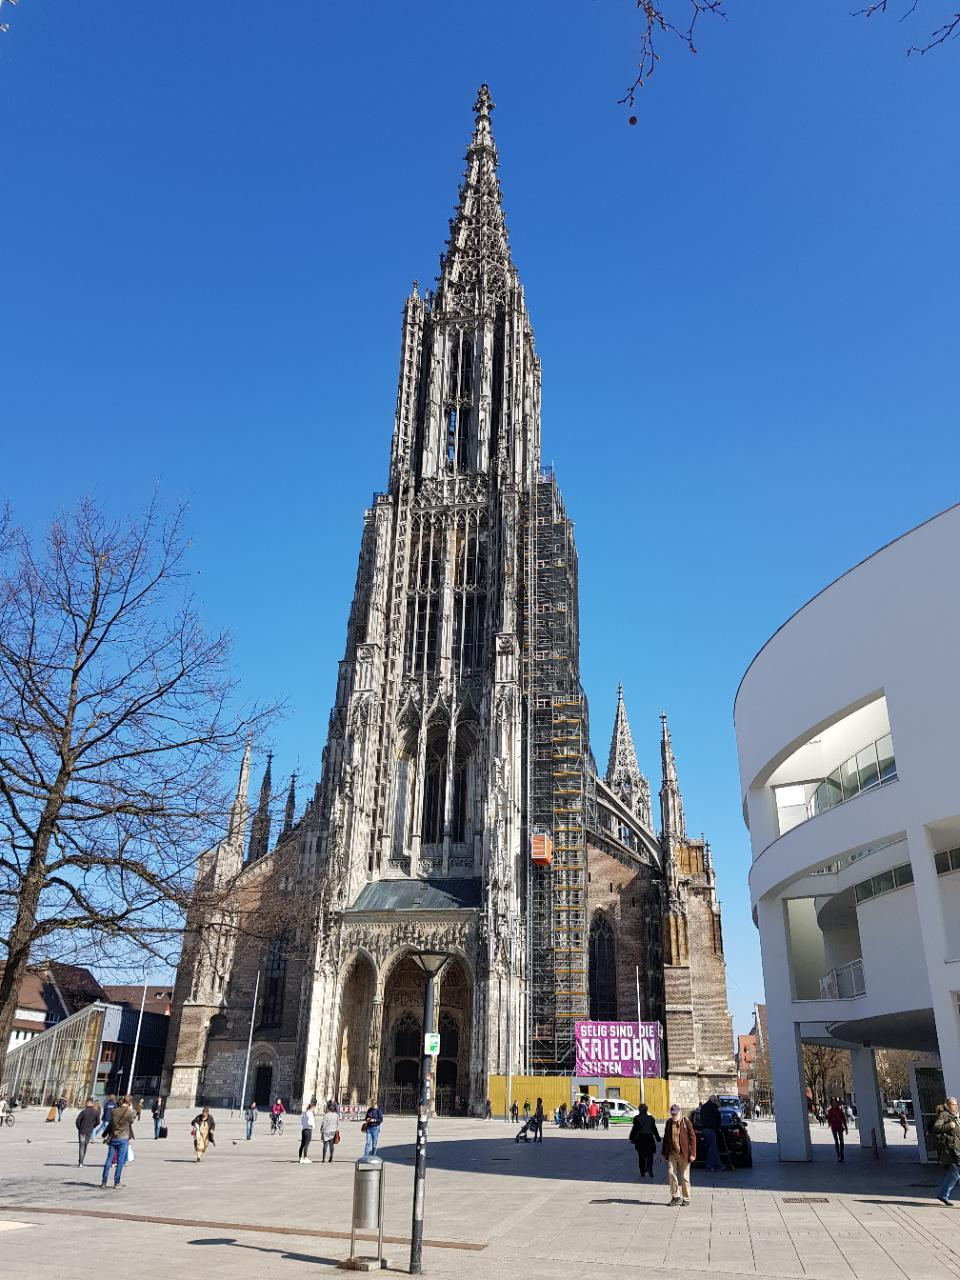
\includegraphics[width=.5\linewidth]{figures/ulm-minster.jpg}
  \caption{Ulm Minster. Photo: wkrauth, CC0, via Wikimedia Commons.}
  \label{fig:jpg}
\end{figure}
\end{ltgexample}

One can also have pictures floating inside text:
\clearpage

\begin{ltgexample}
\begin{floatingfigure}{.33\linewidth}
  \includegraphics[width=.29\linewidth]{example-image-a}
  \caption{A floating figure}
\end{floatingfigure}
\lipsum[2]
\end{ltgexample}

\subsection{Sub Figures}

An example of two sub figures is shown in \zcref{fig:two_sub_figures}.

\begin{ltgexample}
\begin{figure}[!b]
  \centering
  \subfloat[Case I]{\includegraphics[width=.4\linewidth]{example-image-a}%
    \label{fig:first_case}}
  \hfil
  \subfloat[Case II]{\includegraphics[width=.4\linewidth]{example-image-b}%
    \label{fig:second_case}}
  \caption{Example figure with two sub figures.}
  \label{fig:two_sub_figures}
\end{figure}
\end{ltgexample}

\subsection{Figures with tikz}

The \href{https://ctan.org/pkg/pgf}{tikz} package creates graphics programmatically.
This package generates grids and other regular structures.

\begin{ltgexample}
\begin{figure}[ht]
  \centering
  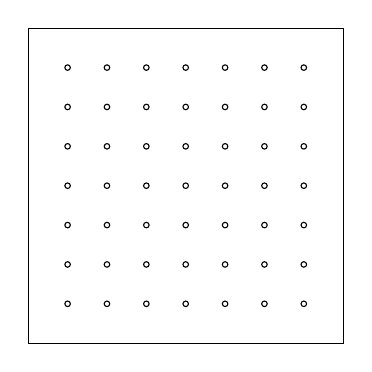
\begin{tikzpicture}
    \draw(0,0) rectangle (4,4);
    \foreach \x in {0.5,1,1.5,2,2.5,3,3.5}
    \foreach \y in {0.5,1,1.5,2,2.5,3,3.5}
    \draw(\x,\y) circle (1pt);
  \end{tikzpicture}
  \caption{A regular grid generated easily with two for loops.}\label{fig:tikz_example}
\end{figure}
\end{ltgexample}

\subsection{Plots with pgfplots}

The \href{https://ctan.org/pkg/pgfplots}{pgfplots} package plots functions directly in \LaTeX{}, similar to MATLAB or gnuplot.
Some visual examples are available in the package documentation\footnote{\url{http://texdoc.net/pkg/pgfplots}}.

\begin{ltgexample}
\begin{figure}[ht]
  \centering
  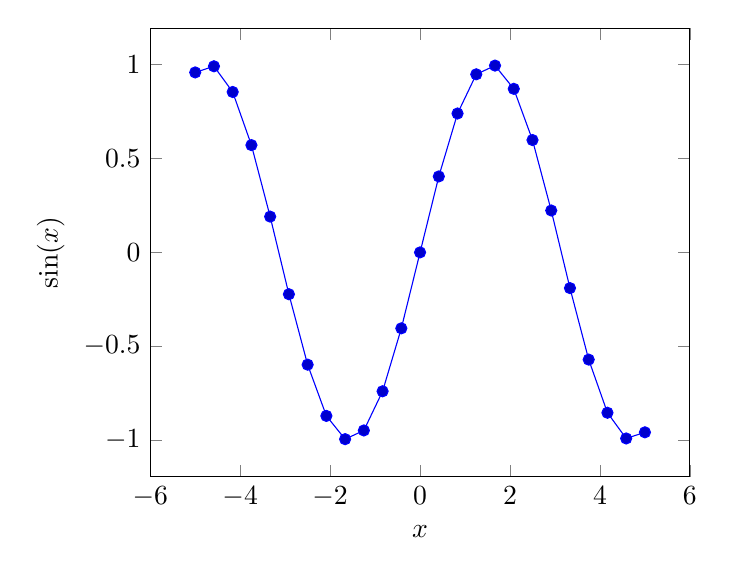
\begin{tikzpicture}
    \begin{axis}[xlabel=$x$, ylabel=$\sin(x)$]
      \addplot {sin(deg(x))};  % Plot the sine function
    \end{axis}
  \end{tikzpicture}
  \caption{Plot of $\sin(x)$ directly inside the figure environment with pgfplots.}
  \label{fig:pgfplots_example}
\end{figure}
\end{ltgexample}

Coordinates can also be given explicitly instead of as a function:
\begin{ltgexample}
\begin{figure}[ht]
  \centering
  \begin{tikzpicture}
    \begin{axis}[xlabel=$x$, ylabel=$y$]
      \addplot coordinates {(0,0) (1,1) (2,4) (3,9)};  % Plot explicit coordinates
    \end{axis}
  \end{tikzpicture}
  \caption{Explicit coordinates plotted with pgfplots.}
  \label{fig:pgfplots_coords}
\end{figure}
\end{ltgexample}

\subsection{Tables}

\begin{ltgexample}
\begin{table}
  \caption{Simple Table}
  \label{tab:simple}
  \centering
  \begin{tabular}{ll}
    \toprule
    Heading1 & Heading2 \\
    \midrule
    One      & Two      \\
    Three    & Four     \\
    \bottomrule
  \end{tabular}
\end{table}
\end{ltgexample}

A table caption goes above the table (\verb|\caption| before the \verb|tabular|), a figure caption below the figure.

Rows and cells can be colored with \verb|\rowcolor| and \verb|\cellcolor| from the \href{https://ctan.org/pkg/colortbl}{colortbl} package, which \href{https://ctan.org/pkg/xcolor}{xcolor} loads with its option \verb|table|.

\begin{ltgexample}
\begin{table}
  \caption{Table with colored cells}
  \label{tab:colored}
  \centering
  \begin{tabular}{ll}
    \toprule
    \rowcolor{gray!20}
    Test & Result                   \\
    \midrule
    A    & \cellcolor{green!20}pass \\
    B    & \cellcolor{red!20}fail   \\
    \bottomrule
  \end{tabular}
\end{table}
\end{ltgexample}

A \verb|\footnote| inside a floating table is lost.
Use \verb|\tablefootnote| from the \href{https://ctan.org/pkg/tablefootnote}{tablefootnote} package instead: it is set as a normal footnote at the bottom of the page.
If the notes should appear directly below the table instead (common in journals), use the \href{https://ctan.org/pkg/threeparttable}{threeparttable} package.

\begin{ltgexample}
\begin{table}
  \caption{Table with a footnote}
  \label{tab:footnote}
  \centering
  \begin{tabular}{ll}
    \toprule
    Heading1 & Heading2\tablefootnote{A footnote inside a table.} \\
    \midrule
    One      & Two                                                \\
    \bottomrule
  \end{tabular}
\end{table}
\end{ltgexample}

\begin{ltgexample}
% Adapted from https://tex.stackexchange.com/a/468994/9075
\begin{table}
  \caption{Table with diagonal line}
  \label{tab:diag}
  \begin{center}
    \begin{tabular}{|l|c|c|}
      \hline
      \diagbox{Row}{Column} & A & B \\
      \hline
      1                     & x & y \\
      \hline
    \end{tabular}
  \end{center}
\end{table}
\end{ltgexample}


\subsection{Tables spanning multiple pages}

The \href{https://ctan.org/pkg/longtable}{longtable} package typesets tables that automatically break across page boundaries.
The header (\verb+\endhead+) and footer (\verb+\endfoot+) rows are repeated on every page; once enough rows are added, the table spans more than one page on its own.

\begin{ltgexample}
\begin{longtable}{|l|l|l|}
  \caption{A sample long table.}\label{tab:long} \\
  \hline
  \multicolumn{1}{|c|}{\textbf{First column}} & \multicolumn{1}{c|}{\textbf{Second column}} & \multicolumn{1}{c|}{\textbf{Third column}} \\ \hline
  \endfirsthead

  \multicolumn{3}{c}{{\bfseries \tablename\ \thetable{} -- continued from previous page}} \\
  \hline
  \multicolumn{1}{|c|}{\textbf{First column}} & \multicolumn{1}{c|}{\textbf{Second column}} & \multicolumn{1}{c|}{\textbf{Third column}} \\ \hline
  \endhead

  \hline \multicolumn{3}{|r|}{{Continued on next page}} \\ \hline
  \endfoot

  \hline\hline
  \endlastfoot

  A & BC & D \\
  A & BC & D \\
  A & BC & D \\
  A & BC & D \\
  A & BC & D \\
  A & BC & D \\
  A & BC & D \\
  A & BC & D \\
  A & BC & D \\
  A & BC & D \\
  A & BC & D \\
  A & BC & D \\
\end{longtable}
\end{ltgexample}

\subsection{Source Code}

The \href{https://github.com/gpoore/minted}{minted} package highlights listings properly.
It uses the \href{http://pygments.org/}{pygments} library, which in turn requires Python.

\begin{ltgexample}
\Zcref{lst:XML} shows source code written in XML.
\Zcref{line:comment} contains a comment.

\begin{listing}[htbp]
  \begin{minted}[linenos=true,escapeinside=||]{xml}
<listing name="example">
  <!-- comment --> |\label{line:comment}|
  <content>not interesting</content>
</listing>
\end{minted}
  \caption{Example XML listing using minted}
  \label{lst:XML}
\end{listing}
\end{ltgexample}

One can also typeset JSON as shown in \zcref{lst:flJSON}.

\begin{ltgexample}
\begin{listing}[htbp]
  \begin{minted}[linenos=true,escapeinside=||]{json}
{
  key: "value"
}
\end{minted}
  \caption{Example JSON listing using minted}
  \label{lst:flJSON}
\end{listing}
\end{ltgexample}

Java is also possible as shown in \zcref{lst:flJava}.

\begin{ltgexample}
\begin{listing}[htbp]
  \begin{minted}[linenos=true,escapeinside=||]{java}
public class Hello {
    public static void main (String[] args) {
        System.out.println("Hello World!");
    }
}
\end{minted}
  \caption{Java code rendered using minted}
  \label{lst:flJava}
\end{listing}
\end{ltgexample}

\subsection{Itemization}

One can list items as follows:

\begin{ltgexample}
\begin{itemize}
  \item Item One
  \item Item Two
\end{itemize}
\end{ltgexample}


One can enumerate items as follows:

\begin{ltgexample}
\begin{enumerate}
  \item Item One
  \item Item Two
\end{enumerate}
\end{ltgexample}


With paralist, one can even have all items typeset after each other and have them clean in the TeX document:

\begin{ltgexample}
\begin{inparaenum}
  \item The first item,
  \item the second item, and
  \item the third item appear in one line.
\end{inparaenum}
\end{ltgexample}

\subsection{Writing in Markdown}\label{sec:markdown}

\ifluatex
  If you are new to \LaTeX{}, you can start by writing your text in Markdown using the \href{https://ctan.org/pkg/markdown}{markdown} package.
  \LaTeX{} then takes care of the typesetting.
  Markdown and \LaTeX{} can be mixed:
  \Zcref{tbl:markdown} is written in Markdown and referenced from \LaTeX{}.
  A whole section can be written in a separate Markdown file included by \verb|\markdownInput|, as \zcref{sec:markdown-file} shows.
  The \href{https://github.com/latextemplates/markdown-latex-quickstart}{markdown-latex-quickstart} shows a complete document written in Markdown.

  \begin{ltgexample}
  \begin{markdown}
Text can be *emphasized* or **bold**, and `code` is set in a monospaced font.
A citation looks like this [@mwe], and here is a footnote.^[This is an inline footnote.]
Referenced footnotes work as well[^detail].

[^detail]: This is a footnote defined at a different place in the text.

- first point
- second point
  - sub-point

1) firstly
2) secondly

| Right | Left | Centered |
|------:|:-----|:--------:|
|    12 | 12   |    12    |
|   123 | 123  |   123    |

: A table written in Markdown {#tbl:markdown}

<#tbl:markdown> shows a table with caption.
Its identifier `{#tbl:markdown}` is referenced by `<#tbl:markdown>`.
\end{markdown}
  \end{ltgexample}
\else
  This example requires \hologo{LuaLaTeX}.
  Compile the document with \hologo{LuaLaTeX} to see it.
\fi

\subsection{Other Features}

\begin{ltgexample}
The words \enquote{workflow} and \enquote{dwarflike} can be copied from the PDF and pasted to a text file.
\end{ltgexample}

\begin{ltgexample}
The symbol for powerset is now correct: $\powerset$ and not a Weierstrass p ($\wp$).

$\powerset({1,2,3})$
\end{ltgexample}

\begin{ltgexample}
Brackets work as designed:
<test>
One can also input backticks in verbatim text: \verb|`test`|.
\end{ltgexample}

Acronyms can be typeset in running text with \verb+\initialism+, which sets them as small caps that blend into the surrounding lowercase text. It is the lightweight alternative to the full acronym and glossary management (\verb+\gls+, with an automatic list of abbreviations) provided by the thesis variants: \verb+\initialism+ only typesets the acronym and does not add it to any list. The macro and the ready-made acronyms (\verb+\OMG+, \verb+\BPEL+, \verb+\BPMN+, \verb+\UML+) are defined in \texttt{commands.tex}, where you can add your own.

\begin{ltgexample}
The \UML is maintained by the \OMG; related standards include \BPEL and \BPMN.
Any acronym can be set inline with \initialism{REST} or \initialism{HTTP}.
\end{ltgexample}


\section{Conclusion and Outlook}
\label{sec:outlook}
\lipsum[1-2]

\subsubsection*{Acknowledgments}

Identification of funding sources and other support, and thanks to individuals and groups that assisted in the research and the preparation of the work should be included in an acknowledgment section, which comes right before the reference section in your document \cite{acmart}.

%%% ===============================================================================
%%% Bibliography
%%% ===============================================================================

\renewcommand{\bibsection}{\section*{References}} % required for natbib to have "References" printed and as section*, not chapter*
% Use natbib compatible splncs04nat style.
% It does provide all features of splncs04.bst, but is developed in a clean way.
% Source: https://github.com/tpavlic/splncs04nat
\bibliographystyle{splncs04nat}
\begingroup
  \microtypecontext{expansion=sloppy}
  \small % ensure correct font size for the bibliography
  \bibliography{paper}
\endgroup

% Enforce empty line after bibliography
\ \\
%
\noindent
All links were last followed on October 5, 2020.

%%% ===============================================================================
%\appendix
%\addcontentsline{toc}{chapter}{APPENDICES}

%\listoffigures
%\listoftables
%%% ===============================================================================

%%% ===============================================================================
%\section{My first appendix}\label{sec:appendix1}
%%% ===============================================================================
\end{document}
